\chapter{Smart Contract Fairness}
\section{Fairness}
\section{Analysis Framework}
\section{Case Study}

%\section{\faircon by Example}\label{Sec_MotivatingExample}

%Because the smart contract can be viewed as a trusted third-party program to perform the trusted
%auctioneer, e-auction smart contracts have been more and more prevalent. As we know, the auction
%in
%the smart contract has been becoming a prominent part of Ethereum. So

In this section, we use an auction contract to illustrate how our approach works in
constructing the intermediate mechanism model and verifying fairness properties.

\begin{example}\label{exp:cryptorome}
	\Cref{CryptoRomeAuction} shows a simplified Ethereum smart contract,
	named \texttt{CryptoRomeAuction}, written in Solidity~\cite{solidity}, taken from
	\texttt{Etherscan}.\footnote{\url{https://etherscan.io/address/0x760898e1e75dd7752db30bafa92d5f7d9e329a81}}
	The contract implements a variant of open English auction for a blockchain-based strategy game,
	where players are allowed to buy virtual lands with cryptocurrencies.
	The auction is given a predefined life cycle parameterized by start and end times.
	A participant can place a bid by sending a message to this contract indicating the value of the bid.
	The address of the participant and the bid amount are stored in variables \texttt{msg.sender} and
	\texttt{msg.value}, respectively.
	The address of the current highest bidder is recorded in \texttt{highestBidder} (Line 9), and a
	mapping \texttt{refunds} is used to keep the contributions of each participant (Line 10) for
	possible refunding later.
	The \texttt{bid()} function (Lines 11--21) is triggered upon receiving the message.
	The bid is rejected if the bid amount is no more than the sum of the current highest bid
	and the minimal increment value \texttt{duration} (Lines 13--15).
	Otherwise, the previous \texttt{highestBidder} gets a refund (Lines 16--18), and the
	\texttt{highestBidder} (Line 19) and \texttt{highestBid} (Line 20) are updated accordingly.
\end{example}

\begin{figure}[t]
	\centering
	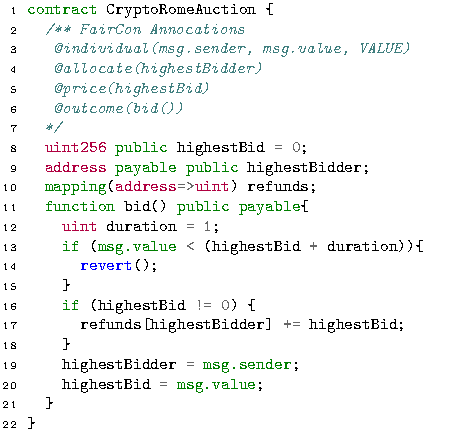
\includegraphics[width=.9\columnwidth]{Figures/Chapter2/auction.pdf}
	\caption{The CryptoRomeAuction Solidity source code.}\label{CryptoRomeAuction}
\end{figure}


%\begin{comment}
%\begin{figure}[t]
%  \small
%  \begin{align*}
%    & \texttt{CryptoRomeAuction} := (msgsender_1, msgvalue_1, \_ ) \\
%    & \quad (msgsender_2, msgvalue_2, \_ ) \\
%    & \quad (msgsender_3, msgvalue_3, \_ ) \\
%    & \quad (msgsender_4, msgvalue_4, \_ ) \\
%    & \quad (msgsender_5, msgvalue_5, \_ ) \\
%    & \quad \texttt{\textbf{assume}}:\; (\mnot (msgvalue_2 < msgvalue_1 + 1)) \mand \\
%    & \quad\quad (\mnot (msgvalue_3 < msgvalue_2 + 1)) \mand \\
%    & \quad\quad (\mnot (msgvalue_4 < msgvalue_3 + 1)) \\
%    & \quad \texttt{\textbf{allocate}}:\; \texttt{\textbf{argmax}}(msgvalue_1,
%    msgvalue_2, msgvalue_3,\\
%    & \quad\quad msgvalue_4,msgvalue_5)\\
%    & \quad \texttt{\textbf{price}}:\; \texttt{\textbf{max}}(msgvalue_1, msgvalue_2,
%    msgvalue_3,\\
%    & \quad\quad msgvalue_4,msgvalue_5)
%\end{align*}%
%  \caption{The mechanism model of CryptoRomeAuction with five bidders.}\label{Crypto_Mechanism}
%\end{figure}
%\end{comment}
\paragraph{Threats to Contract Fairness}
One way that \texttt{CryptoRomeAuction} can become unfair to the participants is through the so
called \emph{shill bidding}~\cite{jenamani2007cheating}---a shill tries to escalate the price
without any intention of buying the item.
This can be induced by either the auctioneer or adversarial participants, and other bidders may
need to pay more as a result.
Occasionally, the shill wins the auction if no other higher bid comes before auction ends.
The item may then be sold again at a later time.

\begin{table}[t]
	\caption{Example instances of CryptoRomeAuction.}\label{tab:example}
	\centering\small
	\begin{tabular}{l|ccc|ccc|ccc}
		\toprule
		& \multicolumn{3}{c|}{Truthful} & \multicolumn{3}{c|}{Untruthful} &
		\multicolumn{3}{c}{Collusion} \\
		\midrule
		Bidder & $p_1$ & $p_2$ & $p_3$ & $p_1$ & $p_2$ & $p_3$ & $p_1$ & $p_2$ & $p_3$ \\
		\midrule
		Valuation  & 3 & 4 & 6 & 3 & 4 & 6 & 3 & 4 & 6\\
		Bid  & 3 & 4 & 6 & 3 & 4 & 5 & 3 & 0 & 4 \\
		Allocation  & \xmark & \xmark & \cmark & \xmark & \xmark & \cmark & \xmark & \xmark & \cmark \\
		Price & 0 & 0 & 6 &  0 & 0 & 5 & 0 & 0 & 4 \\
		Utility  & 0 & 0 & 0 & 0 &  0 & 1 & 0 & 1 & 1 \\
		\bottomrule
	\end{tabular}
\end{table}

Apart from shill bidding, there are a number of other well-studied properties from the game theory
and mechanism design literature, which can be used to evaluate the fairness of an auction.
We use the example instances shown in \cref{tab:example} to demonstrate.
Suppose there are three bidders, $p_1$, $p_2$, and $p_3$, participating in the auction.
Each of them has a valuation of the item, i.e., the item worth three, four, and six units of utility for
$p_1$, $p_2$, and $p_3$, respectively.
The Columns ``Truthful'', ``Untruthful'', and ``Collusion'' in \cref{tab:example} show the
three example scenarios, where the players act truthfully, untruthfully, and collude among
themselves.
The Rows ``Bid'', ``Allocation'', ``Price'', and ``Utility'' show the bids placed, the final
allocation of the item, the clear price, and the utilities obtained by the bidders, respectively.

Same as other first-price auction schemes, \texttt{CryptoRomeAuction} is not \emph{truthful}, i.e.,
bidding truthfully according to one's own valuation of the item is not a dominant strategy.
%Here we show a bidder can cheat in since $CryptoRomeAuction$ cannot have positive incentive to
%drive bidder to truthfully report his bid price.
%Consequently, that cheating bidder could make higher utility while the auction seller suffer the
%loss.
In the ideal truthful scenario, all bidders bid according to their valuations, and $p_3$ wins the
bid with a utility of zero, because the payment equals to his/her valuation of the item.
In another scenario, where $p_3$ bids five (untruthfully), his/her utility would increase by one because
of the lower clear price.
This is called \emph{bid shading}, which only affects the revenue from the auction in this example,
but may affect other participants' utilities in some other cases.
%Further, this cheating benefit may bring negative incentive to other bidders to exercise their
%own truthful bid for this auction as well, which could damage the social welfare realizing in the
%auction.

In the third scenario, $p_2$ and $p_3$ collude in order to gain extra profits.
With full knowledge of each other's valuations, $p_2$ and $p_3$ may decide to form a cartel and
perform bid shading.
One possibility is to have $p_2$ forfeit his/her chance and $p_3$ bids four, and they divide the
profit equally among themselves.
Each of them gains one unit of utility as a result.

%Similar to this example, we also had found cheating problem widely exists in smart contract even
%though there exist many well designed truthful mechanisms available. Unfortunately, many auction
%smart contract try to give a fair illusion to users either via having a promising name or via
%exaggerating its functionality, in order to attract more users involved in the smart contract.
%Meanwhile, the opacity of fairness property of smart contract might make potential users unwilling
%to participate in auction smart contract, thereby decreasing possible social welfare further. Upon
%knowing the fairness properties of auction or other similar type of smart contract,  user may make
%reasonable decision to participate or not in the smart contract.

\paragraph{Checking Fairness Properties}
%\yi{We need to talk about (high-level) how to check fairness properties, such as collusion, on this example automatically.}
Given a mechanism model abstracting the auction settings, the set of fairness properties are
well-defined and can be formally specified based on the model.
The main challenge remains on how to extract the underlying mechanism model from the smart contract
source code.
Now we illustrate how this is done for \texttt{CryptoRomeAuction} in \faircon and outline the process
of automated property checking as well as verification.

%An auction smart contract can be seen as one implementation of some mechanism. To evaluate whether
%auction contract enables truthful incentive or not, we should observe the input and outcome of
%auction related mechanism.
Albeit variations in implementations, all auction contracts share some common components, such as
the bidders' identifiers, their bids, and the allocation as well as clear price rules.
We rely on users to provide annotations for these components directly on the source code, which are
demonstrated on Lines 2--7 in \cref{CryptoRomeAuction}.
Specifically, the annotations specify the bidders' information as a tuple,
``\texttt{@individual(msg.sender,msg.value)}'', indicating the variables used to store the
identifier and the bid value, respectively.
Similarly, ``\texttt{@allocation(highestBidder)}'' and ``\texttt{@price(highestBid)}'' indicate
that the allocation result and the clear price are stored in \texttt{highestBidder} and
\texttt{highestBid}, respectively.
Finally, ``\texttt{@outcome}'' is used to label the function defining the auction allocation logic.

\begin{figure}[t]
	\small
	\begin{align*}
		& \texttt{CryptoRomeAuction} := (msgsender_1, msgvalue_1, \_ ) \\
		& \qquad (msgsender_2, msgvalue_2, \_ ) \\
		& \qquad (msgsender_3, msgvalue_3, \_ ) \\
		& \qquad \texttt{\textbf{assume}}:\; (\mnot (msgvalue_2 < msgvalue_1 + 1)) \mand \\
		& \qquad\qquad (\mnot (msgvalue_3 < msgvalue_2 + 1)) \\
		& \qquad \texttt{\textbf{allocate}}:\; \texttt{\textbf{argmax}}(msgvalue_1,
		msgvalue_2, msgvalue_3)\\
		& \qquad \texttt{\textbf{price}}:\; \texttt{\textbf{max}}(msgvalue_1, msgvalue_2,
		msgvalue_3)
	\end{align*}%
	\caption{The mechanism model of CryptoRomeAuction with three bidders.}\label{Crypto_Mechanism}
\end{figure}

With these labels, we perform symbolic execution~\cite{king1976symbolic} on the \texttt{bid()}
function treating the participants' inputs---\texttt{msg.value}---as \emph{symbolic variables}.
The result of this would be two symbolic expressions for both \texttt{highestBidder} and
\texttt{highestBid}, which symbolically represent the allocation and clear price functions,
respectively.
We can then use these information to synthesize an intermediate mechanism model, shown in
\cref{Crypto_Mechanism}.
The model is specified in a customized language designed for auction and voting contracts.
Details of the language syntax and semantics can be found in \cref{section:mechanism_property}.
At the high level, the model specifies information of the participating individuals and the auction
rules: we consider a bounded model with only three bidders (i.e., $msgsender_1$, $msgsender_2$, and
$msgsender_3$), their bids have to satisfy the constraint specified in the \texttt{assume} clause,
the allocation function is given as ``$\argmax(msgvalue_1,\allowbreak msgvalue_2,\allowbreak
msgvalue_3)$'', and the clear price function is given as ``$\max(msgvalue_1,\allowbreak
msgvalue_2,\allowbreak msgvalue_3)$''.


%In our example as shows in Table \ref{tab:example}, the bid price is the
%input while allocation and payment are parts of the outcome. However, we cannot rely on observing
%the simple input and outcome to reason the fairness property because the valuation of bidder is
%ignored when generating the outcome but useful when analyzing the outcome.
The intermediate mechanism model in \cref{Crypto_Mechanism} has well-defined mathematical
semantics, which can be used to check the desired fairness properties.
We encode both the model and the property with an SMT formula such that a counterexample exists if
and only if the formula is satisfiable.
More details on the encoding can be found in \cref{subsection:property_checking}.
If the formula is unsatisfiable, we are confident that the property holds for the bounded case with
three bidders.
We then attempt to prove the property by instrumenting the contract program with \emph{program
	invariants} encoding the allocation and clear price clauses synthesized previously, but
parameterized by an unbounded number of bidders.
The instrumented program and the property are then passed to a program verification faircon, such as
Dafny~\cite{dafny}, to perform the automated verification.

%Having the valuation in
%analyzing process, taking $CryptoRomeAuction$ as example, firstly we assume there are some players
%that successively update the current highest bidder, then next comes two situation: $M$ $M'$. M is
%ideally truthful for every bidder and we get the utility $u$ of last bidder, the winner in this
%scenario, $M'$ is truthful for every bidder but the last bidder,and we get the utility $u'$ of last
%bidder, also the winner in this scenario, Next comes the comparison between $u$ and $u'$. If $u'$
%is larger than $u$, we can conclude that the contract fails the truthfulness property.  Otherwise,
%we may have some confidence of the truthfulness property of the contract and need to verify it
%using invariant reduction that will discussed in Section \ref{Sec_Method}.











\section{The Analysis Framework for Smart Contract Fairness}
\label{section:mechanism_property}

%\textcolor{red}{Provide a general introduction and overview of the materials/methods and supply essential background information}

In this section, we first provide necessary background and definitions on mechanism models and
fairness properties well studied in the mechanism design
literature~\cite{jackson2014mechanism,nisan2001algorithmic}.
Then we give the abstract syntax and semantics of our mechanism modeling language to support
automated model construction and property checking.

\subsection{Smart Contracts as Mechanism Models}\label{sec:mechanism-model}
Mechanism design is used to design economic mechanisms or incentives to help attain the goals of
different stakeholders who participate in the designated activity.
The goals are mainly related to the outcome that could be described by participants' payoff and
their return in the activity.
We model the logic behind smart contracts with a mathematical object known as the mechanism.
%Largely because of many existing diverse definitions, here we formally describe the mechanism model
%for later understanding fairness property, without the loss of generality.

In a \emph{mechanism model}, we have a finite number of individuals, denoted by $N = \{1, 2, \ldots,
n\}$.
Each individual $i$ holds a piece of private information represented by a \emph{type}, denoted
$\theta_{i} \in \Theta_i$.
Let the types of all individuals be $\theta = (\theta_1, \ldots, \theta_n)$, and the space be
$\Theta = \times_i \Theta_i$.
The individuals report, possibly dishonestly, a \emph{type (strategy) profile} $\report \in \Theta$.
Based on everyone's report, the mechanism model decides an outcome which is specified by an
\emph{allocation function} $d: \Theta \mapsto O$, and a \emph{transfer function} $t: \Theta \mapsto
\mathbb{R}^n$, where $O = \{o_i \in \{0,1\}^n \mid \Sigma_i o_i = 1\}$ is the set of possible
outcomes.

The preferences of an individual over the outcomes are represented using a \emph{valuation function}
$v_i: O \times \Theta_i \mapsto \mathbb{R}$.
Thus, $v_i(o, \theta_i)$ denotes the benefit that individual $i$ of type $\theta_i$ receives from an
outcome $o \in O$, and $v_i(o,\theta_i) > v_i(o',\theta_i)$ indicates that individual $i$ prefers
$o$ to $o'$.
%Individuals may also need to make or receive payment, which is defined by a \emph{transfer
%function}
%$t_i: \Theta \mapsto \mathbb{R}$.
%\yi{TODO: some notations need to be fixed.}
%Having the benefit function $v$ over decisions and transfer
%function $t$, we can easily get the utility $u_i$ of the individual $i$: $ u_i(\theta) =
%v_i(d(\theta), \theta_i) - t_i(d(\theta), \theta_i^s)$. and the social welfare $W$ is sum of all
%individuals' utilities: $ W = \sum_{i=1}^n u_i(\theta)$.
The individual $i$'s utility under strategy profile \report is calculated by subtracting the
payment to be made from the valuation of a certain outcome: $u_i(\report) = v_i(\report,
\theta_i) - t_i(\report)$.